\chapter{Experimentation and Implementation}
\label{chap_imp}

\section*{Introduction}

Semantic Web technologies have immense potential to transform the Internet into a distributed reasoning machine that will not only execute extremely precise searches, but will also have the ability to analyze the data it finds to create new knowledge. Our work uses the Semantic Web tools and infrastructure to show that these semantic technologies are sufficiently mature for expert use, and to solve some of the obstacles to Graphical Representation implementation. 

\section{Work environment}
\label{chap_work}

This section specifies and describes the hardware and software environment that we have used during the implementation of our work.  

\subsection{Hardware configuration}

We were using two computers where we deployed a local Web server in the first machine. The specifications of the computers are displayed in the next table \ref{tablehard}.
%%\caption{Hardware environment}
\begin{table}[H]
\centering
\caption{Hardware environment}
\begin{tabular}{|l|l|l|}
\hline
Specification & Lenovo G500 & Lenovo Z50 \\ 
\hline
RAM & 8GB & 8GB\\ 
\hline
Processor & Intel I3 3120M & Intel I7 4770U \\
\hline
Operating System & Windows 10 Pro & Windows 10 Pro \\ 
\hline
Screen Size & 15"6 & 15"6 \\ 
\hline
Type & Laptop & Laptop \\
\hline
\end{tabular}
\label{tablehard}
\end{table}

\subsection{Software environment }
\label{chap_soft}
In this section, we cite the different tools, languages, softwares and frameworks used in the development of this work.

%%\begin{wrapfigure}[4]{r}{2.5cm}
  %%   \vspace{-5mm}
%%    
\includegraphics[scale=0.2]{nlp}
%%\end{wrapfigure}
\textbf{- Standford CoreNLP} \cite{corenlp}
is a GPL-licensed framework of tools for processing English, Chinese, and Spanish. Includes tools for tokenization (splitting of text into words), part of speech tagging, grammar parsing (identifying things like noun and verb phrases), named entity recognition, and more.\\ 
The choice of the coreNLP over many other NLP tools (e.g: Apache openNLP, GATE, Natural Language Toolkit, etc.) consists to its performance, results and especially its variety of NLP techniques. \\ 

%%\begin{wrapfigure}[3]{r}{1.5cm}
%%     \vspace{-5mm}
%    
\includegraphics[scale=0.3]{owl}
%\end{wrapfigure}
\textbf{- OWL API} \cite{owlapi} is an open source Java API and reference implementation for creating, manipulating and serialising OWL Ontologies. It is now focused on the second version of the Web Ontology Language (OWL2).\\

%%\begin{wrapfigure}[3]{r}{2.5cm}
%%     \vspace{-5mm}
%%    
\includegraphics[width=2.5cm, height=2cm]{jena}
%%\end{wrapfigure}\textbf
{- Apache Jena}\cite{jena} is a Java framework for building Semantic Web applications. It provides a extensive Java libraries for helping developers develop code that handles RDF, RDFS, OWL and SPARQL in line with published W3C recommendations. \\

%\begin{wrapfigure}[3]{r}{2.5cm}
%     \vspace{-5mm}
%    
\includegraphics[width=2.5cm, height=2cm]{netbeans}
%%\end{wrapfigure}
\textbf{- NetBeans} is a powerful integrated development environment (IDE) that is used for developing Java desktop, mobile, and Web applications. It is free, open source, and has a large community of users and developers around the world. \\


%\begin{wrapfigure}[3]{r}{2.5cm}
%     \vspace{-5mm}
%%    
\includegraphics[width=2.5cm, height=2cm]{protetge}
%%\end{wrapfigure}
\textbf{- Protégé} is an Ontology building and editing software with full support of OWL2. It was developed by the Stanford Center for Biomedical Informatics Research at Stanford University, School of Medicine. It is built with JAVA and OWL API. It has desktop and Web version. \\

%\begin{wrapfigure}[3]{r}{2.5cm}
%     \vspace{-5mm}
%    
\includegraphics[width=2.5cm, height=1.2cm]{log4j}
%\end{wrapfigure}
\textbf{- Log4j:} Apache Log4j is a Java-based logging utility. It was originally written by  a Turkish engineer named Ceki Gülcü. It is now a project of the Apache Software Foundation.\\

\textbf{- Hermit:} is reasoner for Ontologies written using the Web Ontology Language (OWL). Given an OWL file, Hermit can determine whether or not the Ontology is consistent, identify subsumption relationships between classes, and much more. It is open-source and released under LGPL licence. 

The version (v1.3.8) of Hermit used with our +Context Ontology is fully compatible with OWLAPI 2.0.0. It is the reason why we had chosen that reasoner along our experimentation because Fact++ and Pellet reasoners were not compatible with the newest version of the OWLAPI and DL queries. \\

%\begin{wrapfigure}[3]{r}{2.5cm}
%     \vspace{-5mm}
%    
\includegraphics[width=2.5cm, height=2cm]{ajaxswing}
%\end{wrapfigure}
\textbf{- AjaxSwing:}  is a Web deployment platform for Java Swing applications. It allows Java desktop applications to run them as Web applications. It is available under commercial license that follows "something-for-something" philosophy, it has a free edition and its source code can be obtained under a small fee. \\

%\begin{wrapfigure}[3]{r}{2.5cm}
%     \vspace{-5mm}
%    
\includegraphics[width=2.5cm, height=2cm]{jsp}
%\end{wrapfigure}
\textbf{- Java Server Page (JSP):} is a text document that contains two types of text: static data, which can be expressed in any text-based format (such as HTML, SVG, and XML), and JSP elements, which construct dynamic content. \\

%\begin{wrapfigure}[3]{r}{2.5cm}
%     \vspace{-5mm}
%    
\includegraphics[width=2.5cm, height=2cm]{tomcat}
%\end{wrapfigure}
\textbf{- Apache Tomcat:} is an open source implementation of the Java Servlet, JavaServer Pages, Java Expression Language and Java WebSocket technologies. The Java Servlet, JavaServer Pages, Java Expression Language and Java WebSocket specifications are developed under the Java Community Process. \\

%\begin{wrapfigure}[3]{r}{2.5cm}
%     \vspace{-5mm}
%    
\includegraphics[width=2.5cm, height=2cm]{jquery}
%%\end{wrapfigure}
\textbf{- jQuery:} is a fast and lightweight JavaScript library. It presents many features including HTML/DOM manipulation, CSS manipulation, HTML event methods, AJAX, etc.

\section{Implementation}
\subsection{Document analysis}

During this step, we use several NLP techniques in order to extract the context and the relations from the document. Although, the process was a bit slow, we managed to determine the main context using Standford's CoreNLP and TextRank (a Java implementation of  the TextRank algorithm \cite{textmark}). The process is executed by extracting the topics (keywords) using CoreNLP by tokenizing the words in every sentence and lemmatizing these keywords. Later, we apply the tokens found into TextRank for more efficient topics extraction. Finally, we used WordNet \cite{wordnet} (a high efficient module that implements a variety of semantic similarity) in order to extract the context.\\

The next step comes in with the relations extraction that we have implemented using openIE \cite{openie} (Open information extraction) a Java implementation of an open IE (Information Extraction) system. This process is also conducted after text processing using NLP. An sample Java code is shown in the listing \ref{openieDefinition} below demonstrating the information extraction procedure.

\newpage

\begin{lstlisting}[captionpos=b, caption=Information extraction process definition in Java, label={openieDefinition},
basicstyle=\footnotesize,frame=single]
 //OpenIE
 Properties props = new Properties();

props.setProperty("annotators", "tokenize,ssplit,pos,lemma,depparse,natlog,openie");

StanfordCoreNLP pipeline = new StanfordCoreNLP(props);

 for (CoreMap sentence : doc.get(CoreAnnotations.SentencesAnnotation.class)) {
      // Get the OpenIE triples for the sentence
      Collection<RelationTriple> triples = sentence.get(NaturalLogicAnnotations.RelationTriplesAnnotation.class);
      // Printing  the triples 

    for (RelationTriple triple : triples ) {
        System.out.println(triple.confidence + "\t" +
            triple.subjectLemmaGloss() + "     \t" +
            triple.relationLemmaGloss() + "    \t" +
            triple.objectLemmaGloss());
    }        
\end{lstlisting}

Considering the context "The French presidential election of 2017" and the following sentence
"Emmanuel Macron is a candidate for the French presidential election 2017." The result of the Information extraction process is shown in the figure \ref{fig_ie} where it shows the minimal developed GUI (Graphical User Interface)  :

\newpage

\begin{figure}[htpb]
\centering
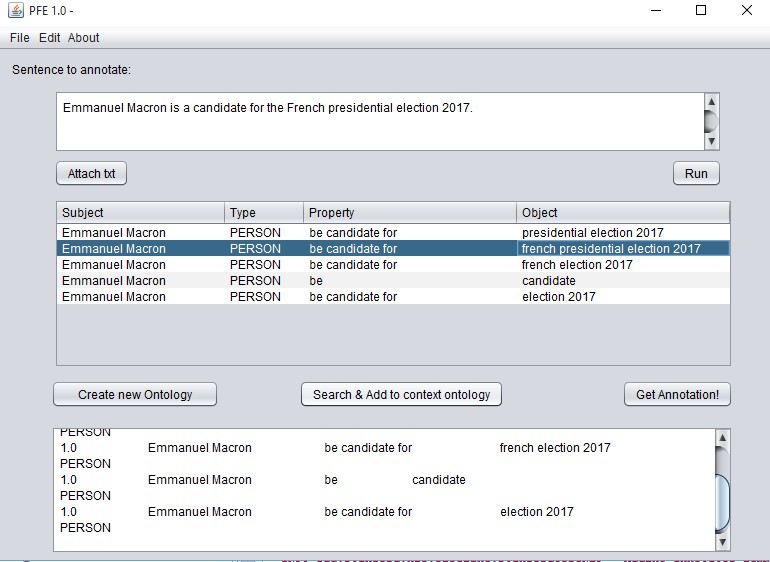
\includegraphics[scale=0.7]{exp1}
\caption{The process of main topics identification }
\label{fig_ie}
\end{figure}

\subsection{Ontology of the Context construction}

Once we have extracted the context and the relations from the desired document, we will construct the Ontology of the context.  \\
The first step is to allow the end user to choose which relations he desires to add to the ontology of the context since the information extraction process is not a very perfect tool so far, like we can see in The figure \ref{fig_const} below.
Once the user chooses the triple to be added to the Ontology of the Context, the application searches Ontologies for the extracted context . If we are able to find the right context, we will simply populate the Ontology that we have acquired during the search process. The population process in this step was implemented through the Hermit reasoner that helped with the search and the extraction of existing relations that we are going to add to the Ontology of the Context. A sample Java code shows how was the population of the context ontology was established is presented in the listing \ref{hermitt} below: \\

\begin{lstlisting}[captionpos=b, caption=Relations search using Hermit reasoner and a DL Query, label={hermitt},
basicstyle=\footnotesize,frame=single]
    public boolean HermitTest(String predicate,String object,OWLOntology ontology) throws ParserException {
    OWLReasoner reasoner = new Reasoner.ReasonerFactory().createReasoner(ontology);
        // Entities are named using IRIs. These are usually too long for use
        ShortFormProvider shortFormProvider = new SimpleShortFormProvider();
        // Create the DLQueryPrinter helper class. This will manage the
        // parsing of input and printing of results
        DLQueryEngine engine = new DLQueryEngine(reasoner, shortFormProvider);
        DLQueryPrinter dlQueryPrinter = new DLQueryPrinter(engine,shortFormProvider);
        // The DL query to search for the relations
        String query =  predicate+" some {"+object+"}";
        System.out.println(query);

        Set<OWLNamedIndividual> individuals = engine
                .getInstances(query, true);
        return dlQueryPrinter.getEntities("Properties", individuals);
    } 
\end{lstlisting}



Otherwise, if we are not able to find the appropriate domain of the Ontology of the context, we will construct a new one. We also gave the end user the opportunity to create a new ontology without looking for an existing Ontology of the context where it is shown in the figure \ref{fig_const}. This process was implemented using OWL API (v4.1.0).  

\begin{figure}[H]
\centering
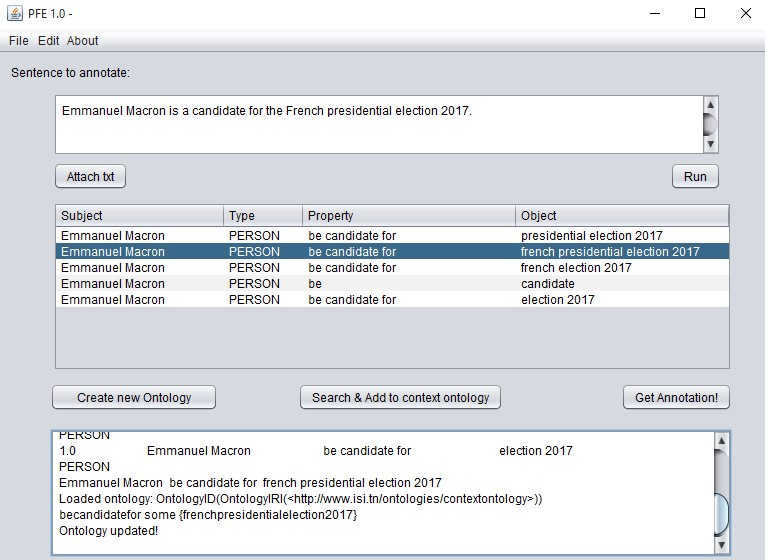
\includegraphics[scale=0.7]{exp2}
\caption{Constructing/populating the context ontology }
\label{fig_const}
\end{figure}
\bigskip

A sample Java code that shows how the population of the context Ontology was established is presented in the listing \ref{consteu} below: \\

\begin{lstlisting}[captionpos=b, caption=Context ontology population definition in Java, label={consteu},
basicstyle=\footnotesize,frame=single]
    //creating ontology manager
    OWLOntologyManager manager = OWLManager.createOWLOntologyManager(); 
    OWLOntology ontology;
            
    ontology = manager.loadOntologyFromOntologyDocument(contextOnt);

    //creating a new idividual from the relation found
    OWLIndividual individual = factory.getOWLNamedIndividual(IRI
            .create(ontologyIRI + "#"+sub.replaceAll("\\s","")));
            
    //matching the individual with the equivalent class    
    OWLClassAssertionAxiom classAssertion = factory.getOWLClassAssertionAxiom(clsAMethodA, individual);

    // validating the changes         
     manager.addAxiom(ontology, classAssertion);       
\end{lstlisting}


The Ontology will be generated in the OWL/XML format that is a bit easy to understand by humans. We chose this format because it is well-formed and structured. Here's a sample of the OWL file after adding the  relation triple into the Ontology of the context. \\


\begin{lstlisting}[captionpos=b, caption=Ontology of the context OWL/XML result, label={consteu},
basicstyle=\footnotesize,frame=none]
    <!-- http://www.isi.tn/ontologies/contextontology#be -->
    <owl:ObjectProperty rdf:about="http://www.isi.tn/ontologies/
    contextontology#be"/>   
    <!-- http://www.isi.tn/ontologies/contextontology#becandidatefor -->
    <owl:ObjectProperty rdf:about="http://www.isi.tn/ontologies/contextontology#becandidatefor"/>
<!-- http://www.isi.tn/ontologies/contextontology#EmmanuelMacron -->
    <owl:NamedIndividual rdf:about="http://www.isi.tn/ontologies/contextontology#EmmanuelMacron">
        <rdf:type rdf:resource="http://www.isi.tn/ontologies/contextontology#PERSON"/>
        <becandidatefor rdf:resource="http://www.isi.tn/
        ontologies/contextontology#frenchpresidentialelection2017"/>
    </owl:NamedIndividual>
    <!-- http://www.isi.tn/ontologies/
    contextontology#FrancoisFillon -->
    <owl:NamedIndividual rdf:about="http://www.isi.tn/ontologies/contextontology#FrancoisFillon">
        <rdf:type rdf:resource="http://www.isi.tn/ontologies/contextontology#PERSON"/>
        <be rdf:resource="http://www.isi.tn/ontologies/contextontology#candidate"/>
    </owl:NamedIndividual>     
\end{lstlisting}

The figure \ref{graphonto} shows the structure of the constructed ontology of the context after the Population process.

\begin{figure}[H]
\centering
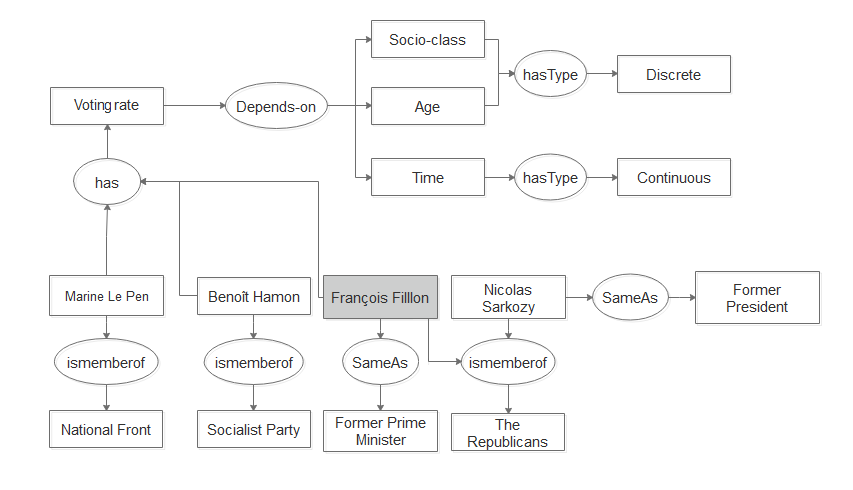
\includegraphics[scale=0.7]{contextOnt}
\caption{Ontology of the Context}
\label{graphonto}
\end{figure}

\subsection{Annotating the document}

The annotation process is the most important step for the on demand graphical representation. The annotation is generated by marking the principal variable and other variable data, accompanied with the relations that already existed in the Ontology of the context. This step is implemented throughout Apache Jena and OWL API in order to extract the different relations from the context ontology.\\ 
This sample java code shows the followed annotation generation process in the listing \ref{annot} below:


\begin{lstlisting}[captionpos=b, caption=Annotation generation definition in Java, label={annot},
basicstyle=\footnotesize,frame=single]
//gathering the individuals from the context ontology
Set<OWLNamedIndividual> inds=ontology.getIndividualsInSignature();
 \\getting the property values from the ontology
for (OWLNamedIndividual ind: inds){
if (!ind.getObjectPropertyValues(ontology).isEmpty()) {
System.out.println(ind.toStringID());

//combining the properties and the subjects found  together.
Map<OWLObjectPropertyExpression, Set<OWLIndividual>> map = ind.getObjectPropertyValues(ontology);
for (Map.Entry<OWLObjectPropertyExpression, Set<OWLIndividual>> entry : map.entrySet())
{
String subject = entry.getKey().toString().replaceAll(ontologyIRI.toString()+"#","");

//Creating an RDF property (Predicate)
Property propAnnot = ResourceFactory.createProperty(entry.getKey().toString());
//creating RDF model of the data found
Resource model1 = RDFmodel.createResource(ind.toStringID().replaceAll("\\s",""))
.addProperty(propAnnot,entry.getValue().toString());
}     
\end{lstlisting}
A sample of the generated RDF/XML annotation is shown in the listing \ref{notaaaa} below:

\begin{lstlisting}[captionpos=b, caption=RDF sample of the generated Annotation, label={notaaaa},
basicstyle=\footnotesize,frame=single]
<rdf:RDF
    xmlns:rdf="http://www.w3.org/1999/02/22-rdf-syntax-ns#"
    xmlns:dc="http://purl.org/dc/elements/1.1/"
    xmlns:graph="http://www.isi.tn/ontologies/contextontology#">
  <rdf:Description rdf:about="http://www.isi.tn/ontologies/contextontology#EmmanuelMacron">
    <graph:becandidatefor>France presidential election 2017</graph:becandidatefor>
  </rdf:Description>
  <rdf:Description rdf:about="http://www.isi.tn/ontologies/contextontology#FrancoisFillon">
    <graph:be>presidential nominee</graph:be>
  </rdf:Description>
  <rdf:Description rdf:about="http://www.isi.tn/ontologies/contextontology#Author">
    <dc:creator>Safoine Benhmida</dc:creator>
  </rdf:Description>
</rdf:RDF>    
\end{lstlisting}

\subsection{Constructing the ontology of graphical models}

As we have mentioned in the previous chapter that the Ontology of graphical models is static, we have constructed it manually using Protégé. A variable as shown in figure \ref{graph} may be continuous or discrete and each type has several graphical representation models. 

\begin{figure}[H]
\centering
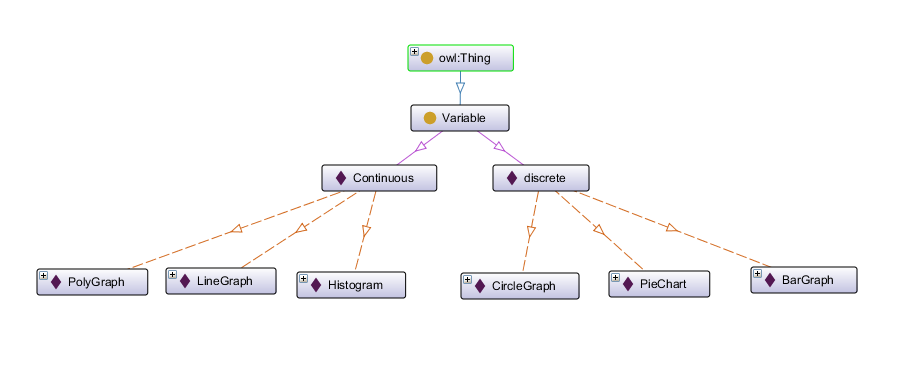
\includegraphics[scale=0.7]{onto}
\caption{Ontology of graphical models structure in Protégé}
\label{graph}
\end{figure}

\subsection{The on demand graphical representation}
The first step of implementing this model is to deploy a Web server that communicates with our based Java application. Thus, the process might seem difficult, we chose to use Apache Tomcat Web server since it is powerful and easy to deploy and most importantly, it is Java implemented. The figure \ref{tomcat} below show's the deployment process of the Web server using JavaSwing.  

\begin{figure}[H]
\centering
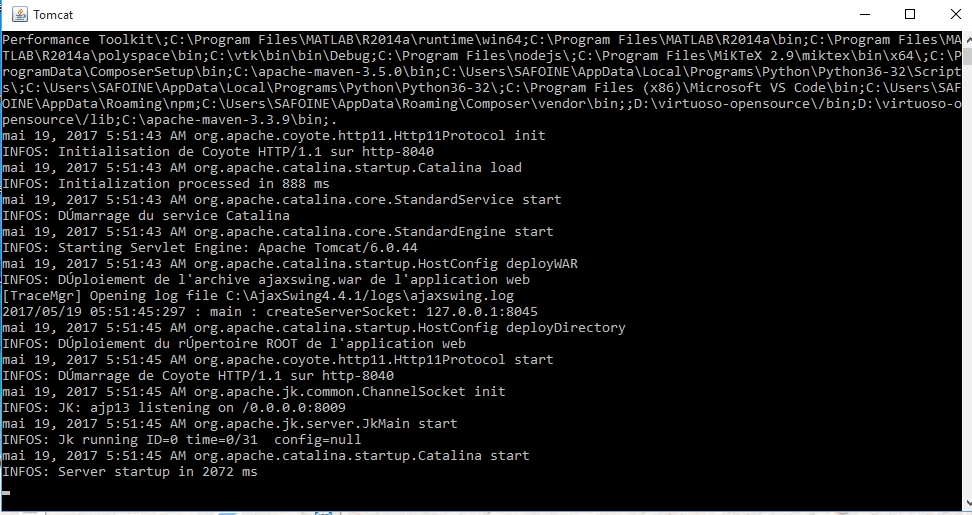
\includegraphics[scale=0.6]{tomcatserver}
\caption{Deploying the Apache Tomcat server}
\label{tomcat}
\end{figure}

During this process, the end user will be able to visualize any variable data that is related to the previously annotated Ontology of the context. Considering the data table  \ref{datatable} associated to the context "Presidential election United States 2016".   
\begin{table}[H]
\centering
\caption{Variable data table}
\label{datatable}
\begin{tabular}{|c|c|c|}
\hline
           & Hilary Clinton & Donald Trump \\ \hline
California & 40\%           & 60\%         \\ \hline
Texas      & 33\%           & 67\%         \\ \hline
New York   & 73\%           & 23\%         \\ \hline
Alabama    & 25\%           & 75\%         \\ \hline
\end{tabular}
\end{table}

The Y-axis element will be also automatically assigned as the principal variable. The variable data in the table will be assigned as a possible X-axis elements. After the analysis of the table is finished, the end user will be able to choose which variable data to visualize according to the available charts that are determined from the variable data criteria and the Ontology of the graphical models. The figure\ref{bargraph} shows the result of a "on demand graphical representation" of the data table \ref{datatable}: 

\begin{figure}[H]
\centering
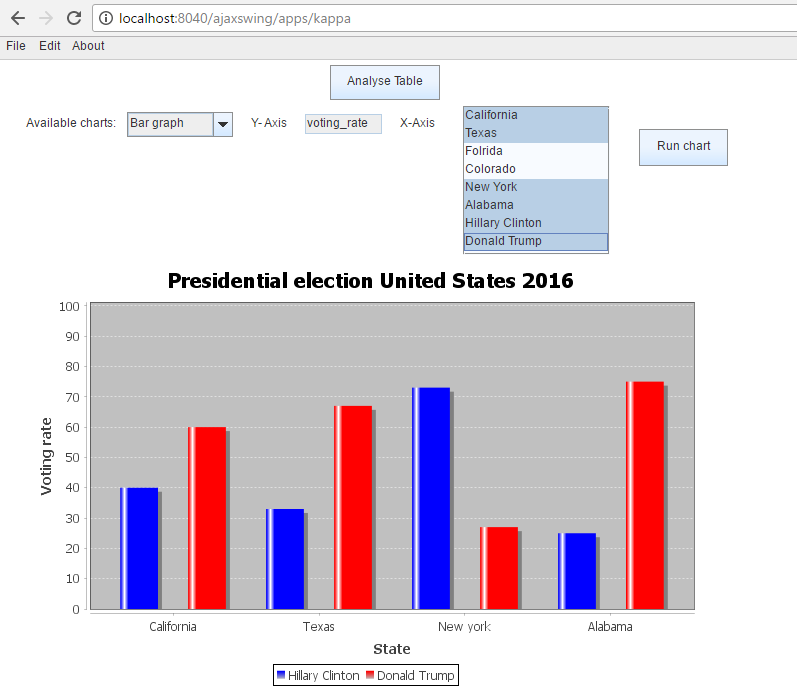
\includegraphics[scale=0.7]{chart1}
\caption{On demand bar graph }
\label{bargraph}
\end{figure}

The figure \ref{bargraph2} below show a result of graphical representation of variable data related to the context "The French presidential election of 2017".

\begin{figure}[H]
\centering
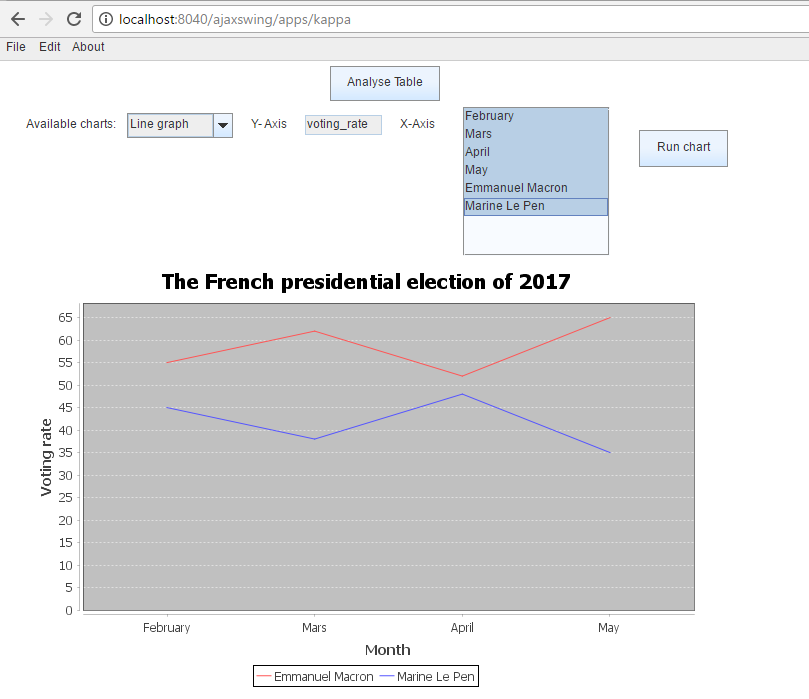
\includegraphics[scale=0.7]{chart2}
\caption{On demand line graph }
\label{bargraph2}
\end{figure}

\section{Conclusion}

Graphic representation is another way of analyzing numerical data. A graph is a sort of chart through which statistical data are represented in the form of lines or curves drawn across the coordinated points plotted on its surface. Graphs enable us in studying the cause and effect relationship between two variables. It helps with measuring the extent of change in one variable when another variable changes by a certain amount. Graphics also enable us in studying both time series and frequency distribution as they give clear account and precise picture of problem. Graphs are also easy to understand and eye catching.

\afterpage{\blankpage}